\startchapter{Channel Modeling}
\label{chapter:Mod}
In this section, I modeled communication channels in the traces. There are two model, guaranteed communication model and in-guaranteed communication model. For both of these two model the communication consist of three stages: 1. channel opening, 2. data exchanging and 3. channel closing.

\section{General Communication Model}   
A communication in this work is happen in a channel. There are 3 main stages of a communication in this model: 1. open the channel, 2. message send/receive, 3. close the channel. Figure \ref{communicationhappen} indicate how communications happen between two ends of both sides of a channel. In the open channel stage, each end need to call its own channel open functions. This open function might be one or more functions which can be channel create function, open function, connect function etc.  In the message send/receive stage, messages are being sent into the channel in one side and received in the other side. In the final channel close stage, the channel delete function, disconnect function, close function etc. will be called. The channel can be reopen again to start new communications after the close stage. However the reopen channel will be treated as a communication cycle.

The operations being concerned in this model are: channel open in sender side, channel open in the receiver side, message send, message receive, channel close in sender side, channel close in receiver side. The number of send and receive function calls for one message do not necessary to be the same. It can be one to one, one to multiple, multiple to one, or multiple to multiple. Both sides of the channel shared the same channel name but different channel handle for its own operations.

\begin{figure}[h]
\centerline{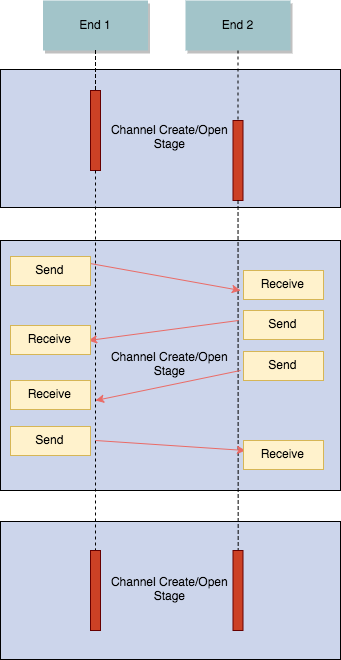
\includegraphics[scale=0.6]{Figures/communicationhappen}}
 \caption{Communication Model}
\label{communicationhappen}
\end{figure}


\section{Data Transfer Model in Different Communication Methods}
I investigate 3 types of communication method, two of them is for internet data transfer, which are TCP and UDP while one of them is for interprocess data transfer, which is named pipe. Based on their properties, they have different data transfer behavior. I summarized their data transfer scenarios in 3 different data transfer models.

\subsection{Data Transfer Model For TCP}
The basic properties of TCP are:
\begin{itemize}
  \item Bytes received in order.
  \item No data lost.
  \item Sender window size is different from receiver’s window size, so segments in the packet can be shuffled.
\end{itemize}
Based on these properties, the data transfer model of it can be summarized in Figure\ref{tcp}
\begin{figure}[h]
\centerline{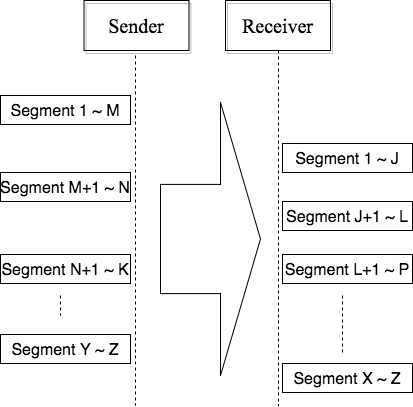
\includegraphics[scale=0.6]{Figures/tcp}}
 \caption{Data Transfer Model for TCP}
\label{tcp}
\end{figure}
\subsection{Data Transfer Model For UDP}
The basic properties of UDP are:
\begin{itemize}
  \item Bytes sent in packet and received in packet, no bytes reorganized.
  \item Packets can lost.
  \item Packets can arrive receiver out of order.
\end{itemize}
Based on these properties, the data transfer model of it can be summarized in Figure\ref{udp}
\begin{figure}[h]
\centerline{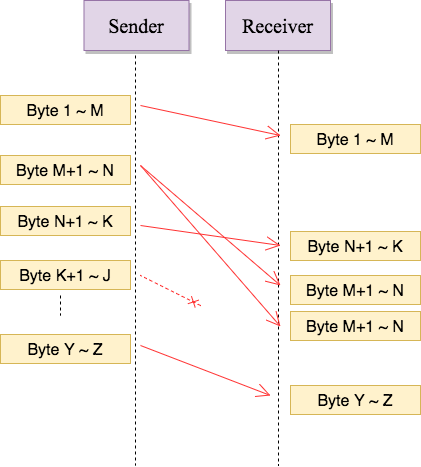
\includegraphics[scale=0.6]{Figures/udp}}
 \caption{Data Transfer Model for UDP}
\label{tcp}
\end{figure}
\subsection{Data Transfer Model For Named Pipe}
The basic properties of TCP are:
\begin{itemize}
  \item Bytes sent in packet and received in packet, no bytes reorganized.
  \item Packets can lost.
  \item Packets can arrive receiver out of order.
\end{itemize}
Based on these properties, the data transfer model of it can be summarized in Figure\ref{namedpipe}
\begin{figure}[h]
\centerline{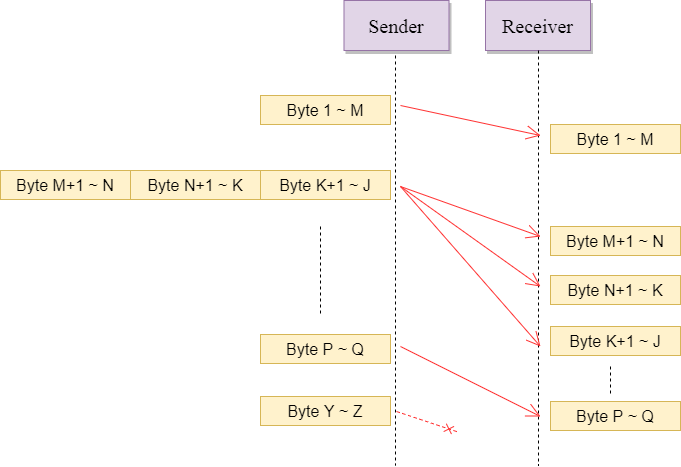
\includegraphics[scale=0.6]{Figures/namedpipe}}
\caption{Data Transfer Model for Named Pipe}
\label{tcp}
\end{figure}
